% !TEX root = ../../现代密码学简介.tex
\chapter{分组密码}
\section{设计密码系统的方法}
我们之前提到如凯撒密码、多表代换密码等经典密码的时候,讲到了破解这些密码的一种方法,就是利用英文中每个字母出现的频率不同。一次一密的方法可以抵御这种破解,原因是对于明文中的每个字符,其移位都是随机的,因此在密文中完全没有明文中字母出现的频率的信息。但是,一次一密的成本又太高,我们有没有什么办法,能尽可能地掩盖在密文中出现的字母频率的信息,来抵御这种频率攻击呢?香农给出了一种解决方法。
\subsection{扩散与混淆}
所谓扩散,指的是如果我们改变明文中的一个字符,加密得到的密文中的多个字符也会得到改变;如果我们改变密文中的一个字符,解密得到的明文中的多个字符也同样会得到改变。因此,明文中一个字符的信息被“扩散”到密文中的多个字符。因此,实现扩散的方法,就可以是用明文中的多个字符去生成密文中的一个字符。\par
扩散是将明文和密文之间的关系变得复杂使我们很难获得密钥,而混淆则是将密钥和密文之间的关系变得复杂。例如,密钥中的一个字符的改变会导致密文中多个字符的改变。因此,即使攻击者通过密文,知道了一些关于明文的统计信息,也很难获得密钥。\par
我们可以发现,凯撒密码的加密方式并没有实现扩散和混淆,因此,它可以被频率攻击轻易破解。
\subsection{置换与代换}
为了实现扩散,常用的方法是置换。也就是说,把输入的一部分与另一部分进行交换,然后输出。置换中最常用的结构为P盒。其接受$m$位二进制输入,$m$位二进制输出。其输出是把输入的比特按一定规则打乱顺序后输出。\par
为了实现混淆,常用的方法是代换。而代换中最常用的结构为S盒。其接受$m$位二进制输入,$n$位二进制输出。因此,其输入共有$2^m$中,输出共有$2^n$种。我们可以把S盒理解成一种查找表。对于$2^m$个输入中的每一种输入,我们可以在这个表中查找到一个$n$位的输出,而且S盒需要保证不同的输入对应的输出也不同。从编程上,我们也可以将此理解成一个长度为$2^m$的数组,它的每个元素为$n$比特的数字。因此,其所占的空间为$n2^m$.
\section{分组密码的定义}
事实上,在非对称密码发展之前,大多数著名的密码体系,其核心都是扩散与混淆。但是,在我们上述谈到扩散与混淆的时候,有一个值得注意的地方:实现扩散与混淆的器件,即P盒与S盒,其接受的都是固定长度的输入。这与我们之前谈到的流密码不同,流密码的输入可以是任意长度的。因此,为了更好地实现扩散与混淆,我们引入了分组密码。\par
分组密码就是一个较好地实现扩散与混淆的密码系统。它的核心思想是分组。首先,将明文分成若干个等长的组,然后对每个组利用密钥依次进行加密,生成等长的密文组。\par
对于分组密码,我们要研究的有:每组内如何根据输入和密钥进行加密,以及各组之间的关系。最简单的方法是各组的输入是之前分好的明文的各个分组,密钥是相同的密钥。但是,也可以使用相对复杂的方法,使加密变得更加复杂(参见“分组密码的运行模式”一节)。\par
由于密文是明文按组生成的,因此,分组密码具有扩散性;而通过采用特别设定的S盒,也可以实现混淆性。\par
这里我们要注意的是,密码学中研究的分组密码,并不仅仅是将明文分组的加密方式。我们之前提到的同步密码,实际上也可以看作是将明文分组进行加密,每个组的长度为其伪随机密钥流的周期。但是,同步流密码依然是逐比特加密,因此,失去了扩散性。所以,只有这个组的每个比特都参与到了密文的生成中的加密方法,才是我们这一章研究的重点。\par
此外,在讨论为分组密码的运行模式,即各组之间的联系之后,我们接下来讨论的DES, IDEA, AES等都是每组内的加密方法。由于分好了组,所以这些密码体制有一个特点,即明文或者密文是固定长度的。
\section{分组密码的设计方法}
之前讲到,对于分组密码,我们要研究的有:每组内如何根据输入和密钥进行加密,以及各组的输入和密钥是什么。本节讨论的是每组内的加密方法。也就是说,在本节内,我们提到的“输入”、“明文”等,都是指被分好组以后的每个组的输入、明文。\par
常见的分组密码有两种核心设计方法:费斯妥密码与SP网络。它们都有一个相同的特点:需要将同一个步骤重复多轮。而在加密过程中,任何核心步骤都是同时需要明文和密钥的信息的。因此,为了保证可靠性,每一轮步骤的输入和密钥都是不一样的。步骤的输入可以根据上一轮的输出来改变,而密钥怎么办呢?这时,就需要\textbf{子密钥}。所谓子密钥,就是根据密钥,生成的不同序列。比如说,某种方法需要16轮步骤,那么,我们就应设计一种算法,使密钥能生成16个子密钥。
\subsection{费斯妥密码}
费斯妥密码每一轮的步骤,接受上一轮的输出$O_{i-1}$为本轮的输入$I_i$, 同时接受子密钥$K_i$, 输出本轮输出$O_i$.\par
首先,将输入的二进制串$O_{i-1}$分成左右两个相等长度的子串$L_{i-1}$和$R_{i-1}$, 然后计算
\begin{gather}
    L_{i}=R_{i-1}\\
    R_{i}=L_{i-1}\oplus F\pth{R_{i-1}, K_i}
\end{gather}

最后输出是把$L_i$和$R_i$拼起来成$O_i$.\par
其中$F\pth{R_{i-1}, K_i}$称为轮函数,是不同具体的加密算法的核心。\par
而由于等式$a\oplus b\oplus b=a$, 因此,其解密过程与加密过程完全相同,只不过需要把子密钥倒着顺序使用。\par
可以用下图形象地理解费斯妥密码(图源wiki):
\begin{figure}[H]
    \centering
    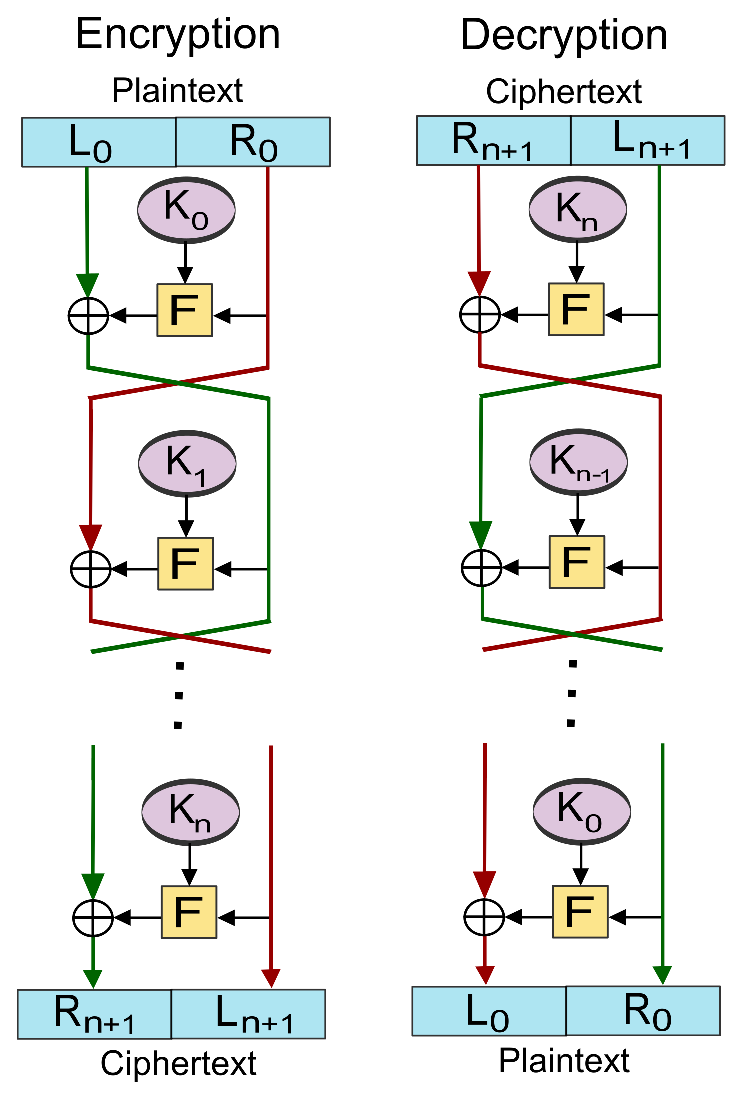
\includegraphics[scale=0.8]{chapters/chapter_3/Feistel.eps}
\end{figure}

值得注意到的一点是,在最后一次输出的时候,不再进行交换,也就是说,输出的并不是$\pth{L_{n+1}, R_{n+1}}$, 而是$\pth{R_{n+1}, L_{n+1}}$.
\subsection{SP网络}
SP网络每轮接受到输入之后,首先,将输入与该轮的子密钥进行异或,然后是对输入再次分组(也就是对分过组的明文的每组内容再次进行分组),接着将每个组通过不同的S盒进行代换,代换后的结果再拼成一个新的串,经过一个P盒的置换进行输出。\par
可以通过下图形象地理解SP网络(图源wiki):
\begin{figure}[H]
    \centering
    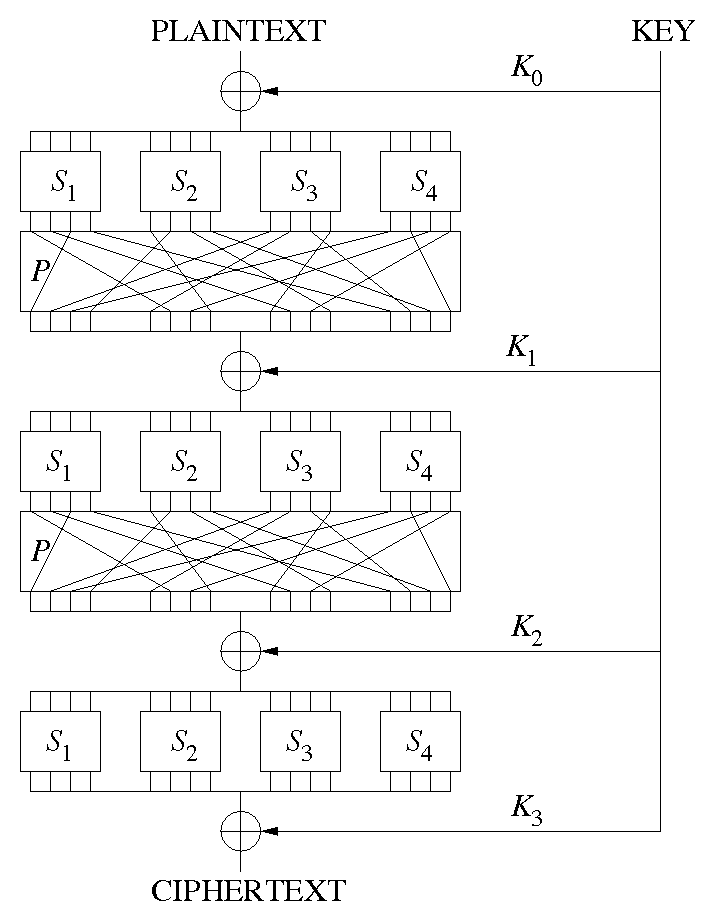
\includegraphics[scale=0.5]{chapters/chapter_3/SPN.png}
\end{figure}
\section{分组密码的运行模式}
上一节讨论了在对明文分好组后,每组内常见的加密方式。本节讨论的,则是组与组之间输入和输出的关系。在这里,假设将明文$M$分成了$m_1, m_2, \ldots, m_n$共$n$个等长的组,在每组内,加密算法为$\E{k}{m}$, 解密算法为$\D{k}{c}$.
\subsection{电码本模式(ECB)}
对于每组,其加密的输入为明文分好的组$m_i$, 密钥为同一个密钥串$k$. 也就是说,
\begin{equation}
c_i=\E{k}{m_i}
\end{equation}

其加密过程如图所示(图源wiki):
\begin{figure}[H]
\centering
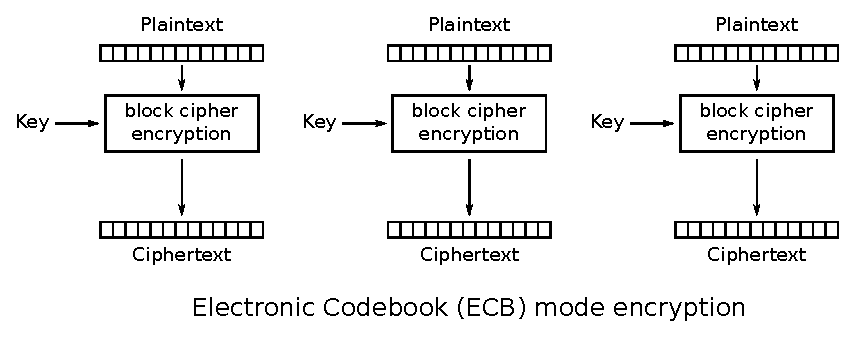
\includegraphics[scale=1]{chapters/chapter_3/ECB.eps}
\end{figure}

ECB模式极不安全。比如说,我想用ECB模式的AES密码体系加密东南大学的校徽:
\begin{figure}[H]
\centering

\includegraphics[width=10em]{chapters/chapter_3/ECB_origin.jpg}
\end{figure}

结果为
\begin{figure}[H]
\centering
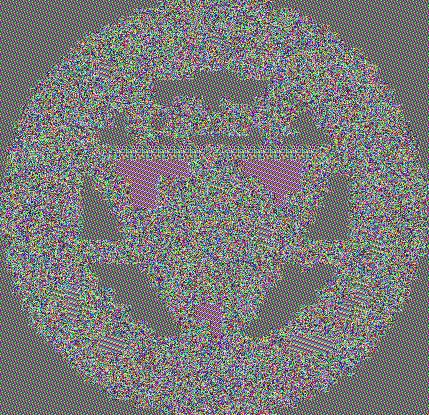
\includegraphics[width=10em]{chapters/chapter_3/ECB_result.jpg}
\end{figure}
\subsection{密码分组链接模式(CBC)}
对于每组,其加密的输入为当前明文组与前一密文组的异或。也就是说,
\begin{equation}
c_i=\E{k}{m_i\oplus c_{i-1}}=\E{k}{m_i\oplus \E{k}{m_{i-1}}}
\end{equation}

对于第一组明文组,由于没有$m_0$, 因此,需要一个初始的二进制串,常记作$IV$, 来与$m_1$异或。\par
其加密过程如图所示(图源wiki):
\begin{figure}[H]
\centering
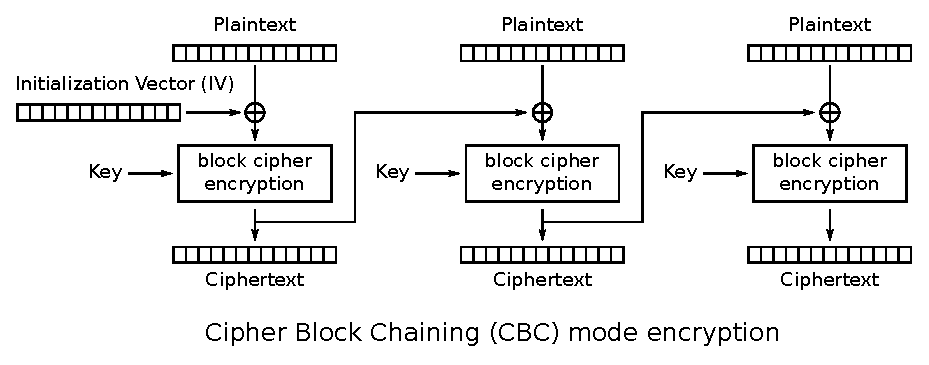
\includegraphics[scale=1]{chapters/chapter_3/CBC.eps}
\end{figure}
\subsection{密码反馈模式(CFB)}
CFB模式需要一个移位寄存器。同时,CFB模式也提供了一个可选的参数$j$, 通常取$j=8$. 其过程如下:\par
对于每组,首先需要进一步分组,使每组的长度为$j$个比特。然后对于每个新分好的组,先将移位寄存器左移$j$个比特,然后将上一组输出的$j$个比特输入到移位寄存器的右边。然后将移位寄存器内存储的二进制串用密钥$k$进行加密,其输出取前$j$个比特与本组的$j$个比特的输入进行异或输出。\par
与CBC类似,处理第一组时移位寄存器内的值也需要一组初始的二进制串$IV$.\par
因此,如果记$H_j(m)$代表取$m$的左边$j$位,$P_i$表示将每组进一步分为的$j$比特的分组,则CFB模式的加密过程可用公式描述为:
\begin{equation}
c_i=H_j\pth{\E{k}{S_{i-1}}}\oplus P_i
\end{equation}
其中$S_i$为移位寄存器的值。移位寄存器的工作方式为
\begin{equation}
S_i=\pth{\pth{S_{i-1} << x}+c_i}\bmod{64}
\end{equation}

如果忽略移位寄存器,其大致的工作原理可由下图表示(图源wiki):
\begin{figure}[H]
\centering
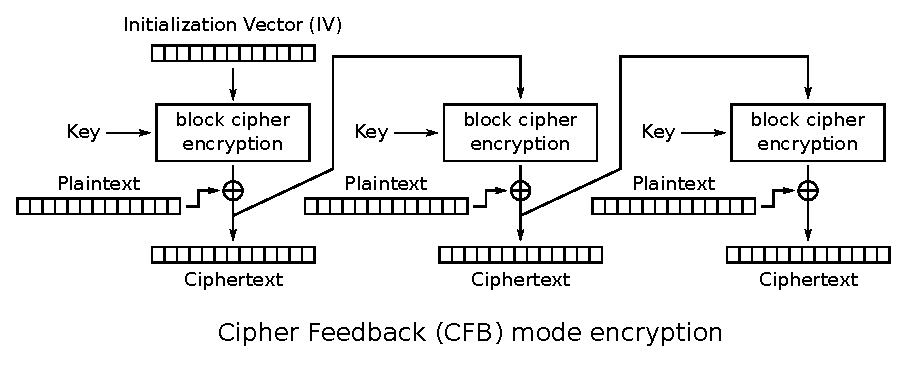
\includegraphics[scale=1]{chapters/chapter_3/CFB.eps}
\end{figure}
\subsection{输出反馈模式(OFB)}
OFB模式与CFB模式极其类似,区别仅在于每组向移位寄存器内的输入为上一组内与明文异或之前的输出。如下图所示(图源wiki):
\begin{figure}[H]
\centering
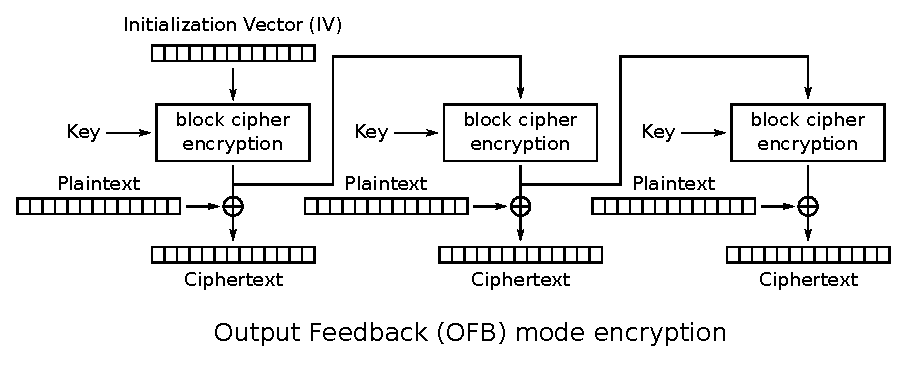
\includegraphics[scale=1]{chapters/chapter_3/OFB.eps}
\end{figure}

从图中可以看到,每组之间传递的数据与明文无关。因此,在OFB中,明文出错只会影响该组的密文,之后的密文都不会被影响。\par
我们如果再仔细看一下OFB的模式图,会发现,事实上,OFB模式把分组密码变成了流密码。真正经过分组密码体系加密的是密钥,而明文则是通过与密钥加密出来的结果异或产生的密文。因此,如果要使OFB模式的安全性高,则要求由分组密码加密出来的密钥为伪随机序列。
\subsection{计数器模式(CTR)}
在借鉴了OFB中本组明文不参与下一组加密的经验之后,引入了CTR模式。在CTR模式中,存在一个计数器函数$f$. 其接受一个初始值,并在每组加密完成后,进行计数,累加到初始值之上。然后每组加密的时候,只需要将该函数的返回值输入分组加密算法中,输出值与当前明文组异或产生密文输出。\par
其过程如图所示(图源wiki):
\begin{figure}[H]
\centering
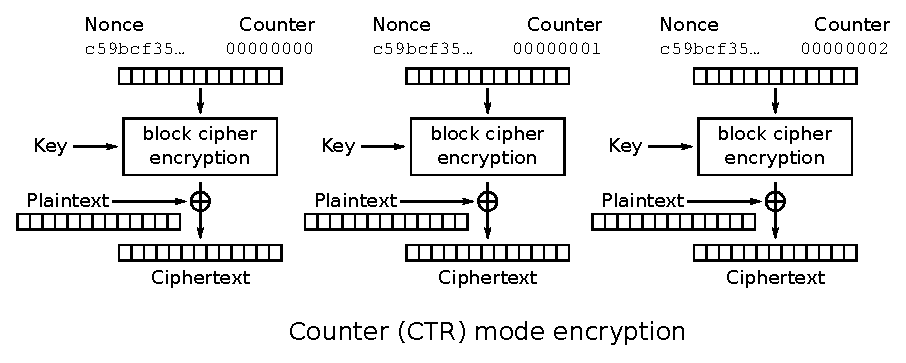
\includegraphics[scale=1]{chapters/chapter_3/CTR.eps}
\end{figure}

根据上图,我们可以发现CTR的独一无二的好处:可以并行加密。其每组加密不需要上组的任何信息,只需要该组对应的计数器值即可。
\section{DES}
接下来,我们讨论的是,在每组内的分组加密算法。\par
DES是最著名的分组密码之一。我们可以先大致地讨论其算法,然后再讨论其一些性质。
\subsection{算法与代码}
DES采用了费斯妥密码的结构,并对它进行了一定的改进。之前我们提到的费斯妥密码,可以改进的地方有其最开始的输入、子密钥、轮函数以及最后的输出。因此,我们分别就上述几个方面来分块解释DES的算法。
\subsubsection{主体:费斯妥密码}
首先,我们介绍DES的主体——费斯妥密码。正如之前说的,费斯妥密码为一个步骤的多轮操作。其核心公式为
\begin{gather}
    L_{i}=R_{i-1}\\
    R_{i}=L_{i-1}\oplus F\pth{R_{i-1}, K_i}
\end{gather}
其中,$L_{i-1}, R_{i-1}$为上一轮输出的左右两半,$L_i, R_i$为本轮输出的左右两半,$F\pth{R_{i-1}, K_i}$为轮函数,$K_i$为本轮的子密钥。\par
此外,从数学上可以证明,费斯妥密码的解密过程的核心公式也是上述公式,只不过使用的密钥的顺序与加密正好相反。\par
DES密码一共进行16轮这样的步骤,并且其输入为64位二进制串,子密钥为48位二进制串(实际操作中是56位的二进制串,其中有8位是校验位不用于加密过程),输出为64位二进制串。\par
其C程序代码如下:
\begin{prove}
\begin{verbatim}
bitset<64> round(bitset<64> input, bitset<48> ki)
{
    bitset<64> output;
    bitset<32> previousLeftPart;
    bitset<32> leftPart;
    bitset<32> rightPart;
    
    for (int i = 0; i < 32; i++)
        previousLeftPart[31 - i] = input[63 - i];
    
    for (int i = 0; i < 32; i++)
        leftPart[31 - i] = input[31 - i];
    
    rightPart = previousLeftPart ^ F(leftPart, ki);
    
    for (int i = 0; i < 32; i++)
        output[63 - i] = leftPart[31 - i];
    
    for (int i = 32; i < 64; i++)
        output[63 - i] = rightPart[63 - i];

    return output;
}
\end{verbatim}
\end{prove}
\subsubsection{费斯妥密码的轮函数}
在费斯妥密码的轮函数这里,实际上是采用了SP网络的思想,也就是将轮函数的输入经过S盒的代换来混淆和P盒的置换来扩散。\par
轮函数接受32位的输入和48位的子密钥。首先,将32位的输入扩充成48位的二进制串(可以理解成通过了一个32位到48位的S盒,称为选择扩展运算E),然后将其逐比特与48位的子密钥异或,输出的48位二进制串作为一个48位到32位的S盒的输入。接着,将S盒输出的32位二进制串经过一个P盒(称为置换运算P)输出。\par
这里的48位到32位的S盒实际上是由8个6位到4位的S盒组成。其将输入的48位分组输入,然后再分组输出。\par
因此,轮函数所做的事情有:将32位的输入扩展成48位,进行异或,输入S盒,输入P盒。其C程序代码如下:
\begin{prove}
    \begin{verbatim}
int E[] = {32,  1,  2,  3,  4,  5,
            4,  5,  6,  7,  8,  9,
            8,  9, 10, 11, 12, 13,
           12, 13, 14, 15, 16, 17,
           16, 17, 18, 19, 20, 21,
           20, 21, 22, 23, 24, 25,
           24, 25, 26, 27, 28, 29,
           28, 29, 30, 31, 32,  1};

int S_BOX[8][4][16] = {
    {
        {14,4,13,1,2,15,11,8,3,10,6,12,5,9,0,7},
        {0,15,7,4,14,2,13,1,10,6,12,11,9,5,3,8},
        {4,1,14,8,13,6,2,11,15,12,9,7,3,10,5,0},
        {15,12,8,2,4,9,1,7,5,11,3,14,10,0,6,13}
    },
    {
        {15,1,8,14,6,11,3,4,9,7,2,13,12,0,5,10},
        {3,13,4,7,15,2,8,14,12,0,1,10,6,9,11,5},
        {0,14,7,11,10,4,13,1,5,8,12,6,9,3,2,15},
        {13,8,10,1,3,15,4,2,11,6,7,12,0,5,14,9}
    },
    {
        {10,0,9,14,6,3,15,5,1,13,12,7,11,4,2,8},
        {13,7,0,9,3,4,6,10,2,8,5,14,12,11,15,1},
        {13,6,4,9,8,15,3,0,11,1,2,12,5,10,14,7},
        {1,10,13,0,6,9,8,7,4,15,14,3,11,5,2,12}
    },
    {
        {7,13,14,3,0,6,9,10,1,2,8,5,11,12,4,15},
        {13,8,11,5,6,15,0,3,4,7,2,12,1,10,14,9},
        {10,6,9,0,12,11,7,13,15,1,3,14,5,2,8,4},
        {3,15,0,6,10,1,13,8,9,4,5,11,12,7,2,14}
    },
    {
        {2,12,4,1,7,10,11,6,8,5,3,15,13,0,14,9},
        {14,11,2,12,4,7,13,1,5,0,15,10,3,9,8,6},
        {4,2,1,11,10,13,7,8,15,9,12,5,6,3,0,14},
        {11,8,12,7,1,14,2,13,6,15,0,9,10,4,5,3}
    },
    {
        {12,1,10,15,9,2,6,8,0,13,3,4,14,7,5,11},
        {10,15,4,2,7,12,9,5,6,1,13,14,0,11,3,8},
        {9,14,15,5,2,8,12,3,7,0,4,10,1,13,11,6},
        {4,3,2,12,9,5,15,10,11,14,1,7,6,0,8,13}
    },
    {
        {4,11,2,14,15,0,8,13,3,12,9,7,5,10,6,1},
        {13,0,11,7,4,9,1,10,14,3,5,12,2,15,8,6},
        {1,4,11,13,12,3,7,14,10,15,6,8,0,5,9,2},
        {6,11,13,8,1,4,10,7,9,5,0,15,14,2,3,12}
    },
    {
        {13,2,8,4,6,15,11,1,10,9,3,14,5,0,12,7},
        {1,15,13,8,10,3,7,4,12,5,6,11,0,14,9,2},
        {7,11,4,1,9,12,14,2,0,6,10,13,15,3,5,8},
        {2,1,14,7,4,10,8,13,15,12,9,0,3,5,6,11}
    }
};

int P[] = {16,  7, 20, 21,
           29, 12, 28, 17,
            1, 15, 23, 26,
            5, 18, 31, 10,
            2,  8, 24, 14,
           32, 27,  3,  9,
           19, 13, 30,  6,
           22, 11,  4, 25};

bitset<4> S_boxi(bitset<6> input, int i)
{
    int row = 2 * input[5] + input[0];
    int column = 8 * input[4] + 4 * input[3] + 2 * input[2]
                 + input[1];
    int outputint = S_BOX[i][row][column];
    bitset<4> output(outputint);

    return output;
}
           
bitset<32> S_box(bitset<48> input)
{
    bitset<32> output;
    bitset<6> SiInput[8];

    for (int i = 0; i < 8; i++)
    {
        for (int j = 0; j < 6; j++)
            SiInput[i][5 - j] = input[47 - (j + i * 6)];

        bitset<4> SiOutput = S_boxi(SiInput[i], i);

        for (int j = 0; j < 4; j++)
            output[31 - (j + i * 4)] = SiOutput[3 - j];
    }

    return output;
}
           
bitset<32> F(bitset<32> rightPart, bitset<48> ki)
{
    bitset<32> output;
    bitset<48> expandedInput;

    for (int i = 0; i < 48; i++)
        expandedInput[47 - i] = rightPart[32 - E[i]];

    bitset<48> S_boxInput = expandedInput ^ ki;
    bitset<32> S_boxOutput = S_box(S_boxInput);

    for (int i = 0; i < 32; i++)
        output[31 - i] = S_boxOutput[32 - P[i]];

    return output;
}
    \end{verbatim}
\end{prove}
\subsubsection{费斯妥密码的最初输入}
DES加密算法接受64位明文输入,DES解密算法接受64位密文输入。为了更好地实现扩散性,首先,需要将输入的64位二进制串经过一个P盒。在DES算法中,这个P盒被称作初始置换IP. 随后,将经过置换后的64位二进制串作为费斯妥密码的输入。\par
其C程序代码如下:
\begin{prove}
    \begin{verbatim}
int IP[] = {58, 50, 42, 34, 26, 18, 10, 2,
            60, 52, 44, 36, 28, 20, 12, 4,
            62, 54, 46, 38, 30, 22, 14, 6,
            64, 56, 48, 40, 32, 24, 16, 8,
            57, 49, 41, 33, 25, 17, 9,  1,
            59, 51, 43, 35, 27, 19, 11, 3,
            61, 53, 45, 37, 29, 21, 13, 5,
            63, 55, 47, 39, 31, 23, 15, 7};

bitset<64> getInitialPermutation(bitset<64> input)
{
    bitset<64> initialPermutation;

    for (int i = 0; i < 64; i++)
        initialPermutation[63 - i] = input[64 - IP[i]];

    return initialPermutation;
}
    \end{verbatim}
\end{prove}
\subsubsection{费斯妥密码的最终输出}
之前我们再三强调,费斯妥密码的最后一轮输出后,还要将左右两边互换,也就是最终输出为$\pth{R_{16}, L_{16}}$而非$\pth{L_{16}, R_{16}}$. 此外,为了使DES的加密和解密算法能尽可能复用,我们将输出再经过一个P盒才形成最终的DES的输出。其中,输出时经过的P盒要是输入时P盒的逆,被称为逆初始置换$\mathrm{IP}^{-1}$. 这样的话,我们假设明文为$m$, 密文为$c$, 中间的费斯妥密码部分(包括最后的左右交换),加密为$f(x)$, 解密为$f^{-1}(x)$. 那么,DES加密的过程为
\[c=\mathrm{IP}^{-1}\pth{f\pth{\mathrm{IP}\pth{m}}}\]

而只需要把中间的$f$换成$f^{-1}$:
\begin{align*}
    &\mathrm{IP}^{-1}\pth{f^{-1}\pth{\mathrm{IP}\pth{c}}}\\
    =&\mathrm{IP}^{-1}\pth{f^{-1}\pth{\mathrm{IP}\pth{\mathrm{IP}^{-1}\pth{f\pth{\mathrm{IP}\pth{m}}}}}}\\
    =&\mathrm{IP}^{-1}\pth{f^{-1}\pth{f\pth{\mathrm{IP}\pth{m}}}}\\
    =&\mathrm{IP}^{-1}\pth{\mathrm{IP}\pth{m}}\\
    =&m
\end{align*}
即可实现解密。\par
因此,DES输出包括交换费斯妥密码输出的左右位置,以及通过逆初始置换$\mathrm{IP}^{-1}$. 其C程序代码如下:
\begin{prove}
    \begin{verbatim}
int IP_1[] = {40, 8, 48, 16, 56, 24, 64, 32,
              39, 7, 47, 15, 55, 23, 63, 31,
              38, 6, 46, 14, 54, 22, 62, 30,
              37, 5, 45, 13, 53, 21, 61, 29,
              36, 4, 44, 12, 52, 20, 60, 28,
              35, 3, 43, 11, 51, 19, 59, 27,
              34, 2, 42, 10, 50, 18, 58, 26,
              33, 1, 41,  9, 49, 17, 57, 25};

bitset<64> exchangeLeftAndRight(bitset<64> input)
{
    bitset<64> output;

    for (int i = 0; i < 32; i++)
        output[63 - i] = input[31 - i];

    for (int i = 32; i < 64; i++)
        output[63 - i] = input[95 - i];

    return output;
}

bitset<64> getInversePermutation(bitset<64> input)
{
    bitset<64> output;

    for (int i = 0; i < 64; i++)
        output[63 - i] = input[64 - IP_1[i]];

    return output;
}
    \end{verbatim}
\end{prove}
\subsubsection{密钥的处理}
对于输入的密钥,我们需要让其生成16个子密钥。类似于费斯妥密码,这里的16次生成也是同样的步骤循环16次。但首先,我们需要处理的是DES算法输入的64位密钥。\par
DES算法输入的64位密钥中,通常包含8位奇偶校验位。首先,我们将奇偶校验位去除,得到56位的真正的密钥。然后,再将其通过一个P盒(称为置换选择1:PC\_1),作为接下来生成子密钥的算法的输入。\par
其C程序代码为:
\begin{prove}
\begin{verbatim}
int PC_1[] = {57, 49, 41, 33, 25, 17, 9,
               1, 58, 50, 42, 34, 26, 18,
              10,  2, 59, 51, 43, 35, 27,
              19, 11,  3, 60, 52, 44, 36,
              63, 55, 47, 39, 31, 23, 15,
               7, 62, 54, 46, 38, 30, 22,
              14,  6, 61, 53, 45, 37, 29,
              21, 13,  5, 28, 20, 12,  4};

bitset<56> getKeyPermutation(bitset<64> key)
{
    bitset<56> output;

    for (int i = 0; i < 56; i++)
        output[55 - i] = key[64 - PC_1[i]];

    return output;
}
\end{verbatim}
\end{prove}
\subsubsection{子密钥的生成}
由于DES算法中的费斯妥密码部分一共需要16轮循环,因此共需要16个子密钥。在DES算法中,采用了同一个步骤循环16次的方式生成子密钥。该步骤接受56位二进制串的输入,生成48位的子密钥和56位的输出。其包含两个操作:循环移位和置换选择2。\par
之前我们提到,在DES密码算法中,加密和解密仅有的区别就是子密钥的使用顺序。因此,这种区别就体现在了子密钥生成的算法上。\par
在循环移位步骤中,其接受56位的输入,然后将这56位的二进制串分为左右两个28位的二进制串。并在每一轮中,将这两个二进制串分别循环移位。加密过程是左循环移位,解密过程是右循环移位,并且每一轮移动的位数不同。\par
在循环移位操作完成后,将左右两个二进制串重新拼成一个56位的二进制串作为输出和下一轮操作的输入,同时,再将56位的二进制串经过一个56位到48位的S盒(称为置换选择2: PC\_2), 作为本轮的子密钥。\par
其C程序代码为:
\begin{prove}
\begin{verbatim}
enum ShiftStyle {
    leftShift,
    rightShift
};

int shiftBits[] = {1, 1, 2, 2, 2, 2, 2, 2, 1, 2, 2, 2, 2, 
                    2, 2, 1};
int inverseShiftBits[] = {0, 1, 2, 2, 2, 2, 2, 2, 1, 2, 2, 
                            2, 2, 2, 2, 1};

int PC_2[] = {14, 17, 11, 24,  1,  5,
               3, 28, 15,  6, 21, 10,
              23, 19, 12,  4, 26,  8,
              16,  7, 27, 20, 13,  2,
              41, 52, 31, 37, 47, 55,
              30, 40, 51, 45, 33, 48,
              44, 49, 39, 56, 34, 53,
              46, 42, 50, 36, 29, 32};

bitset<56> shiftKey(bitset<56> key, int round, 
                    ShiftStyle shiftStyle)
{
    bitset<56> output;

    bitset<28> previousLeftPart;
    for (int i = 0; i < 28; i++)
        previousLeftPart[27 - i] = key[55 - i];

    bitset<28> previousRightPart;
    for (int i = 0; i < 28; i++)
        previousRightPart[27 - i] = key[27 - i];

    int *shift;
    switch (shiftStyle)
    {
        case leftShift:
            shift = shiftBits;
            break;
            
        case rightShift:
            shift = inverseShiftBits;
            break;
            
        default:
            break;
    }
    
    bitset<28> leftPart;
    bitset<28> rightPart;
    int shiftBit = shift[round];

    switch (shiftStyle)
    {
        case leftShift:
            for (int i = 0; i < 28; i++)
            {
                leftPart[27 - i] = previousLeftPart[(27 - i
                                     - shiftBit + 28) % 28];
                rightPart[27 - i] = previousRightPart[(27 - i
                                     - shiftBit + 28) % 28];
            }
            break;
            
        case rightShift:
            for (int i = 0; i < 28; i++)
            {
                leftPart[27 - i] = previousLeftPart[(27 - i
                                     + shiftBit + 28) % 28];
                rightPart[27 - i] = previousRightPart[(27 - i
                                     + shiftBit + 28) % 28];
            }
            break;
            
        default:
            break;
    }

    for (int i = 0; i < 28; i++)
        output[55 - i] = leftPart[27 - i];

    for (int i = 28; i < 56; i++)
        output[55 - i] = rightPart[55 - i];

    return output;
}

bitset<48> getSubkey(bitset<56> key, int round, 
                     ShiftStyle shiftStyle)
{
    bitset<48> output;

    for (int i = 0; i < 48; i++)
        output[47 - i] = key[56 - PC_2[i]];

    return output;
}
\end{verbatim}
\end{prove}
\subsubsection{DES加密和解密}
以上就是DES密码的每个组成部分。我们可以把它们组合起来,实现DES的加密和解密。其C程序代码如下:
\begin{prove}
\begin{verbatim}
bitset<64> DES_ENC(bitset<64> plainText, bitset<64> key)
{
    bitset<64> cipher;
    bitset<64> roundInput = getInitialPermutation(plainText);
    bitset<64> roundOutput;
    bitset<56> permutatedKey = getKeyPermutation(key);
    bitset<56> previousShiftOutput = shiftKey(permutatedKey, 0,
                                                 leftShift);
    for (int i = 0; i < 16; i++)
    {
        bitset<48> subkey = getSubkey(previousShiftOutput, i, 
                                        leftShift);
        roundOutput = round(roundInput, subkey);
        roundInput = roundOutput;
        previousShiftOutput = shiftKey(previousShiftOutput, 
                                        i + 1, leftShift);
    }
    cipher = getInversePermutation(
                exchangeLeftAndRight(roundOutput));
    return cipher;
}

bitset<64> DES_DEC(bitset<64> cipher, bitset<64> key)
{
    bitset<64> plainText;
    bitset<64> roundInput = getInitialPermutation(cipher);
    bitset<64> roundOutput;
    bitset<56> permutatedKey = getKeyPermutation(key);
    bitset<56> previousShiftOutput = shiftKey(permutatedKey, 0, 
                                                rightShift);
    for (int i = 0; i < 16; i++)
    {
        bitset<48> subkey = getSubkey(previousShiftOutput, i, 
                                        rightShift);
        roundOutput = round(roundInput, subkey);
        roundInput = roundOutput;
        previousShiftOutput = shiftKey(previousShiftOutput, 
                                        i + 1, rightShift);
    }
    plainText = getInversePermutation(
                    exchangeLeftAndRight(roundOutput));
    return plainText;
}
\end{verbatim}
\end{prove}
\subsection{多重DES}
我们可以看出,DES密码使用了费斯妥密码,并且局部也使用了SP网络,这样使这种分组密码的安全性较高。在几乎30年的大量研究之后,已知对DES的最好的实用攻击仍然只是对密钥空间的穷举搜索。但是,DES使用的密钥在去除奇偶校验位之后的实际长度只有56位,在如今的计算机水平下,变得十分容易破解。在2017年,通过计算机更是创下了在25秒内破解DES的记录。\par
鉴于此,人们选择了多重DES加密。如二重DES加密:使用一个112位的密钥$K$, 将其分为$K_1$和$K_2$两个56位的密钥。如果记$\mathrm{E}_k\pth{m}$为DES的加密过程,$\mathrm{D}_k\pth{m}$为DES的解密过程,那么,其加密过程为
\[\mathrm{E}_{K_1}\pth{\mathrm{E}_{K_2}\pth{m}}\]
解密过程为
\[\mathrm{D}_{K_2}\pth{\mathrm{D}_{K_1}\pth{c}}\]

而如今最常用的是二密钥的三重DES,简称为TDES密码。其使用一个112位的密钥$K$, 将其分为$K_1$和$K_2$两个56位的密钥,其加密过程为
\[\mathrm{E}_{K_1}\pth{\mathrm{D}_{K_2}\pth{\mathrm{E}_{K_1}\pth{m}}}\]
解密过程为
\[\mathrm{D}_{K_1}\pth{\mathrm{E}_{K_2}\pth{\mathrm{D}_{K_1}\pth{c}}}\]
\subsection{结构特性}
除了DES的密钥过短,从数学角度来看,DES密码拥有一些结构特性,也降低了其破解的难度。
\subsubsection{互补特性}
对于二进制串$m$, 如果我们记$\overline{m}$为$m$按位取补,并用$\mathrm{DES}_k\pth{m}$表示通过密钥$k$, 二进制串$m$的DES加密的密文,那么,我们可以证明:
\begin{equation}
\mathrm{DES}_{\overline{k}}\pth{\overline{m}}=\overline{\mathrm{DES}_k\pth{m}}
\end{equation}

因此,在使用穷举搜索破解时,可以使工作量减少一半。假设有一个使用已知明文攻击的攻击者,他可以选择明密文对$\pth{M, C}$和$\pth{\overline{M}, C^*}$. 那么,在所有的$2^{56}$个可能的密钥,也就是$2^{55}$对互补的密钥二进制串中,他只需要每对互补的二进制串中取一个,一共搜索$2^{55}$个密钥。对于每个尝试的密钥$l$, 如果$\mathrm{DES}_{l}\pth{M}=C$或$\overline{C^*}$, 就说明密钥是$l$或$\overline{l}$.
\subsubsection{弱密钥与半弱密钥}
在多重DES加密的过程中,有一些密钥十分危险。比如说弱密钥:
\begin{Definition}
在DES加密的过程中,如果存在一个密钥$w$, 使得
\begin{equation}\label{weakKey}
\mathrm{E}_w\pth{\mathrm{E}_w\pth{m}}=m
\end{equation}

则称$w$为弱密钥。
\end{Definition}

从另一个角度解释公式\ref{weakKey}, 也就是说,
\begin{equation}
\mathrm{E}_w\pth{m}=\mathrm{D}_w\pth{m}
\end{equation}

而我们之前提到,DES密码的加密与解密过程唯一的区别就是子密钥的使用顺序。据此我们可以很容易地构造弱密钥$w$, 也就是使其生成子密钥时加密与解密循环移位的结果相同即可。在56位的密钥中,共有4个弱密钥。\par
此外,还有半弱密钥对
\begin{Definition}
在DES加密的过程中,如果存在一对密钥$w_1, w_2$, 使得
\begin{equation}
\mathrm{E}_{w_1}\pth{\mathrm{E}_{w_2}\pth{m}}=m
\end{equation}

则称$w_1, w_2$为一对半弱密钥。
\end{Definition}

在3DES密码中,如果选取的两个密钥是一对半弱密钥,后果不堪设想。在56位的密钥中,共有6对半弱密钥。
\section{IDEA}
\subsection{符号说明}
在介绍IDEA之前,首先,先介绍一些IDEA加密过程中用到的数学符号。
\begin{itemize}
\item 逐比特异或$\oplus$\par
$m_1\oplus m_2$即将两个16位的二进制串逐比特异或。
\item 模$2^{16}$整数加法$\boxplus$\par
即对于16位二进制数$m_1, m_2$, $m_1\boxplus m_2=\pth{m_1+m_2}\bmod{2^{16}}$.
\item 模$2^{16}+1$整数乘法$\odot$\par
即对于16为二进制数$m_1, m_2$, $m_1\odot m_2=\pth{m_1\cdot m_2}\bmod{\pth{2^{16}+1}}$.\par
这里特别指出,如果$m_1=00\ldots 0$, 应把$m_1$看作$2^{16}$. 这是由于$2^{16}+1=65537$为素数,故由数论知识我们可以知道,模$2^{16}+1$的非零整数乘法构成一个群,即所有非零整数都有逆元。此外,这样也可以保证输出一定不会超过16位。由于$2^{16}+1$为素数,所以如果$\pth{m_1m_2}\bmod{\pth{2^{16}+1}}=0$, 则表明$m_1$或$m_2$必然是$2^{16}+1$的倍数。而$m_1, m_2$均为16位字符串,所以这是不可能的。
\end{itemize}
\subsection{轮结构}
和其他分组密码类似,IDEA也是采用了多次重复轮结构的步骤。其轮结构如图所示(图源wiki):
\begin{figure}[H]
\centering
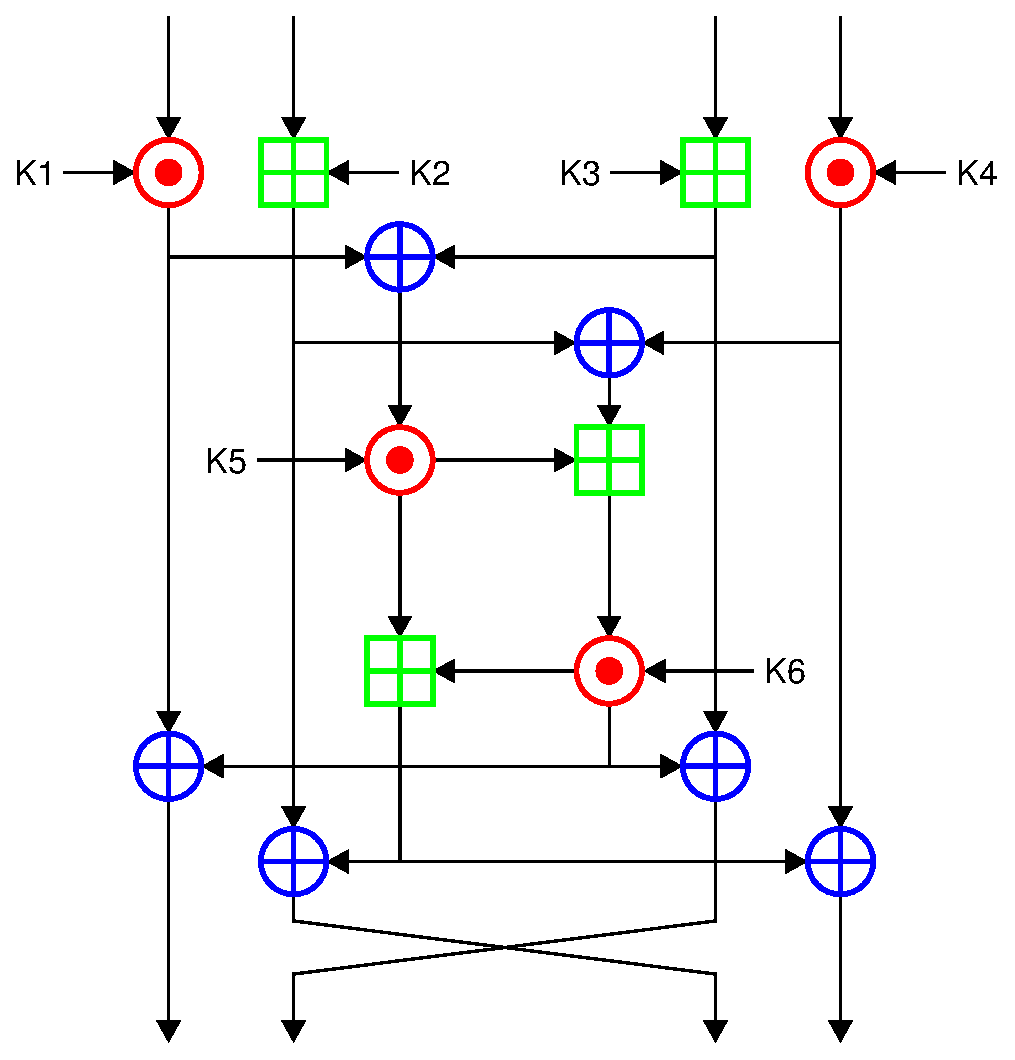
\includegraphics[scale=0.5]{chapters/chapter_3/IDEA_round.eps}
\end{figure}

在每一轮中,一共需要输入6个16位的子密钥,并且输入为4组16位的二进制串,输出也为4组16位的二进制串。
\subsection{加密过程}
IDEA加密算法接受64位明文和128位密钥。对于密钥,将其通过一个子密钥生成器生成48个16位的子密钥用于8轮轮结构,加上6个16位的子密钥用于输出变换。\par
首先,将64位明文分成4组等长的子串,然后输入轮结构中。在经过8轮轮结构后,将输出的结构通过如图所示的输出变换(图源wiki),得到密文。
\begin{figure}[H]
\centering
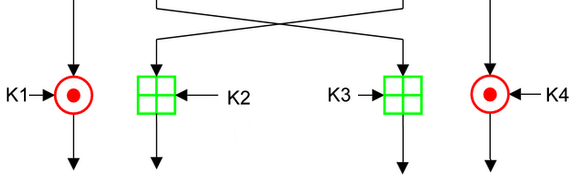
\includegraphics[scale=0.5]{chapters/chapter_3/IDEA_output.png}
\end{figure}

而子密钥的生成算法则相对比较直接:\par
前8个子密钥$Z_1, Z_2, \ldots, Z_8$直接在加密密钥中依次选取。然后,将加密密钥循环左移$52$位,再依次取接下来的8个子密钥。以此类推,直到52个子密钥全部生成。
\section{AES}
\subsection{输入与输出}
AES密码接受的明文与密钥的长度可独立选择128位、192位或256位。这些选择之间的区别仅仅在于加密运算的轮数以及子密钥的调度不同。但是在AES密码标准中,明文长度固定为128位,密钥长度可以选择为128, 192或256位,分别叫做AES-128, AES-192和AES-256.\par
在处理过程中,我们对明文和密钥进一步分组。AES密码的每个步骤的处理单位是一个“字节”,即8个比特。因此,我们将明文和密钥分成每组长度为8比特的分组,每个8比特的明文分组称为一个“状态”。\par
对于由字节组成的明文,我们第二次进行分组,使其分成4个等长的分组,记明文的每个分组的长度为$N_b$ (在实际操作中明文总是128位,因此$N_b=4$). 此外,我们也记以字节为单位的密钥的长度除以$4$为$N_k$ ($N_k$的可能取值为$4, 6, 8$). 我们如果假定由字节组成的明文是一个长度为$4N_b$的数列$\{M_n\}$, 那么,我们可以按下表的顺序填充分组:
\begin{table}[H]
\centering
\begin{tabular}{c|c|c|c}\hline
$M_0$&$M_4$&$\cdots$&$M_{4N_b-3}$\\\hline
$M_1$&$M_5$&$\cdots$&$M_{4N_b-2}$\\\hline
$M_3$&$M_6$&$\cdots$&$M_{4N_b-1}$\\\hline
$M_4$&$M_7$&$\cdots$&$M_{4N_b}$\\\hline
\end{tabular}
\end{table}

由明文的分组组成的阵列称为状态阵列。在AES的实际过程中,都是对状态阵列进行操作。最终的密文就是从状态序列中,按写入顺序拿出的序列。\par
因此,在加密的输入阶段,我们要做的事是将明文和密钥按字节分组,然后将明文再填入状态阵列中。在加密的输出阶段,就是将密文从状态阵列中读出,再变成以比特为单位的二进制串(但事实上,明文或密文的按字节分组可以直接在填入状态阵列的时候做。因此,我们只需要实现比特串向字节串的转化用于密钥,而不需要实现字节串向比特串的转化)。在解密阶段,我们要做的也是同样的步骤,只不过是明文和密文对调。\par
此环节的C程序代码如下:
\begin{prove}
\begin{verbatim}
void bitToByte(bitset<128> inputBits, bitset<8> outputBytes[64])
{
    for (int byte = 0; byte < 64; byte++)
        for (int bit = 0; bit < 8; bit++)
            outputBytes[byte][bit] = inputBits[8 * byte + bit];
}

void bitToState(bitset<128> input, bitset<8> state[4][4])
{
    for (int column = 0; column < 4; column++)
        for (int row = 0; row < 4; row++)
            for (int bit = 0; bit < 8; bit++)
                state[row][column][bit] = input[32 * column
                                                + 8 * row + bit];
}

void stateToBit(bitset<8> state[4][4], bitset<128> &output)
{
    for (int column = 0; column < 4; column++)
        for (int row = 0; row < 4; row++)
            for (int bit = 0; bit < 8; bit++)
                output[32 * column + 8 * row + bit]
                    = state[row][column][bit];
}
\end{verbatim}
\end{prove}
\subsection{轮函数}
AES的轮函数由4个计算部件组成,分别为字节代换(ByteSub), 行移位(ShiftRow), 列混合(MixColumn), 密钥加(AddRoundKey).
\subsubsection{字节代换}
字节代换可以看作一个128位到128位的S盒。其接受输入状态阵列,然后对状态阵列实现S盒的操作。\par
在C程序实现里,加密过程中,S盒为\verb`bitset<8> S_box[16][16]`; 解密过程中,S盒为\verb`bitset<8> Inv_S_Box[16][16]`. 这两个S盒的值在AES中是固定的,其生成方式可以看后面的数学论证部分。\par
其C程序实现如下:
\begin{prove}
\begin{verbatim}
void SubByte(bitset<8> state[4][4], CryptoMode cryptoMode)
{
    bitset<8> (*crypto_S_box)[16];

    switch (cryptoMode)
    {
        case Enc:
            crypto_S_box = S_box;
            break;
            
        case Dec:
            crypto_S_box = Inv_S_Box;
            break;
            
        default:
            break;
    }
    
    for (int row = 0; row < 4; row++)
        for (int column = 0; column < 4; column++)
        {
            bitset<8> previousValue = *(*(state + row) + column);
            int S_box_row = previousValue[7] * 8
                                + previousValue[6] * 4
                                    + previousValue[5] * 2
                                        + previousValue[4];
            int S_box_column = previousValue[3] * 8
                                + previousValue[2] * 4
                                    + previousValue[1] * 2
                                        + previousValue[0];
            *(*(state + row) + column)
                = crypto_S_box[S_box_row][S_box_column];
        }
}
\end{verbatim}
\end{prove}
\subsubsection{行移位}
在之前处理数据的时候,我们提到把明文分为4组。每组可以看作一行,每行包括$N_b$个字节。\par
所谓行移位,就是将各行进行循环移位,不同的行的位移量不同。第一行不移位,第二行左移$C_1$, 第三行左移$C_2$, 第四行左移$C_3$. $C_1, C_2, C_3$都与$N_b$有关。\par
在解密时,只需要反向循环移位即可。\par
其C程序实现如下:
\begin{prove}
\begin{verbatim}
int shiftBytes[4] = {0, 1, 2, 3};

void ShiftRows(bitset<8> state[4][4], CryptoMode cryptoMode)
{
    for (int row = 0; row < 4; row++)
    {
        bitset<8> previousRow[4];
        for (int column = 0; column < 4; column++)
            previousRow[column] = state[row][column];
        switch (cryptoMode)
        {
            case Enc:
                for (int column = 0; column < 4; column++)
                    state[row][column]
                        = previousRow[(column
                                       - shiftBytes[row] + 4) % 4];
                break;
                
            case Dec:
                for (int column = 0; column < 4; column++)
                    state[row][column]
                        = previousRow[(column
                                       + shiftBytes[row]) % 4];
                break;
                
            default:
                break;
        }
    }
}
\end{verbatim}
\end{prove}
\subsubsection{列混合}
该步骤是对状态阵列的每一列进行变换。为了方便我们理解以及后面的数学论证,我们将这一步理解成矩阵乘法。由于每一列共有4个元素,因此,我们可以把它看作一个四维列向量$(a_0, a_1, a_2, a_3)^{\mathrm{T}}$. 其输出也为4位列向量$(b_0, b_1, b_2, b_3)^{\mathrm{T}}$.\par
在加密过程中,其计算方法为
\begin{equation}
\pth{\begin{array}{c}b_0\\b_1\\b_2\\b_3\end{array}}=\pth{\begin{array}{cccc}02&03&01&01\\01&02&03&01\\01&01&02&03\\03&01&01&02\end{array}}\pth{\begin{array}{c}a_0\\a_1\\a_2\\a_3\end{array}}
\end{equation}

在解密过程中,其计算方法为
\begin{equation}
\pth{\begin{array}{c}a_0\\a_1\\a_2\\a_3\end{array}}=\pth{\begin{array}{cccc}0e&0b&0d&09\\09&0e&0b&0d\\0d&09&0e&0b\\0b&0d&09&0e\end{array}}\pth{\begin{array}{c}b_0\\b_1\\b_2\\b_3\end{array}}
\end{equation}

这里要特别指出的是,在矩阵相乘时,每一项之间的乘法并不是我们平时用到的十进制乘法。这种乘法遵循特定的乘法表。在C程序实现中,我们发现,只需要使用与01, 02, 03, 09, 0b, 0d, 0e的乘法。因此,对于这7个数,我们各有一张长度为256的表,用于与一个字节对应的比特(共$2^8=256$种)相乘($a_0, a_1, a_2, a_3$都是一个字节)的结果。\par
其C程序实现如下:
\begin{prove}
\begin{verbatim}
bitset<8> *M[4][4] = {
    {Mul_02, Mul_03, Mul_01, Mul_01},
    {Mul_01, Mul_02, Mul_03, Mul_01},
    {Mul_01, Mul_01, Mul_02, Mul_03},
    {Mul_03, Mul_01, Mul_01, Mul_02}
};

bitset<8> *Inv_M[4][4] = {
    {Mul_0e, Mul_0b, Mul_0d, Mul_09},
    {Mul_09, Mul_0e, Mul_0b, Mul_0d},
    {Mul_0d, Mul_09, Mul_0e, Mul_0b},
    {Mul_0b, Mul_0d, Mul_09, Mul_0e}
};

void MixColumns(bitset<8> state[4][4], CryptoMode cryptoMode)
{
    bitset<8>* (*crypto_M)[4][4];

    switch (cryptoMode)
    {
        case Enc:
            crypto_M = &M;
            break;
            
        case Dec:
            crypto_M = &Inv_M;
            break;
            
        default:
            break;
    }
    for (int column = 0; column < 4; column++)
    {
        bitset<8> previousColumn[4];
        for (int row = 0; row < 4; row++)
            previousColumn[row] = state[row][column];
        for (int row = 0; row < 4; row++)
        {
            state[row][column] = 0;
            for (int i = 0; i < 4; i++)
                state[row][column]
                    ^= *(*(*(*crypto_M + row) + i)
                        + previousColumn[row].to_ulong());
        }
    }
}
\end{verbatim}
\end{prove}
\subsubsection{密钥加}
在我们输入密钥之后,首先会通过密钥编排算法,得到若干长度为$N_b$的轮密钥。密钥加即为将轮密钥与当前的状态阵列逐比特异或。解密时再次异或即可。\par
其C程序实现如下:
\begin{prove}
\begin{verbatim}
void AddRoundKey(bitset<8> state[4][4], bitset<32> ki[4])
{
    for (int row = 0; row < 4; row++)
        for (int column = 0; column < 4; column++)
            for (int bit = 0; bit < 8; bit++)
                state[row][column][bit]
                    = ki[row][column * 4 + bit]
                        ^ state[row][column][bit];
}
\end{verbatim}
\end{prove}
\subsubsection{轮函数总的步骤}
在每一轮中,对当前的状态阵列,轮函数依次进行字节代换、行移位、列混合和与当前轮密钥的密钥加,最后输出。\par
在最后一轮中,不进行列混合。
\subsection{密钥编排算法}
之前我们讲到,我们输入的密钥会通过密钥编排算法变成若干长度为$N_b$的轮密钥。密钥编排算法分为密钥扩展和轮密钥选取两个部分。\par
考虑到每个轮密钥长度都为$N_b$, 假设我们需要进行$N_r$轮,则一共需要$N_b\pth{N_r+1}$长度的密钥。因此,我们首先需要将输入的密钥扩展成对应长度的扩展密钥。\par
然后,第一轮轮密钥取扩展密钥的第一个$N_b$长度个字,第二轮轮密钥取接下来的$N_b$长度个字,以此类推。\par
\subsubsection{密钥扩展算法}
在密钥扩展算法中,我们需要用到$N_r$个轮常数\verb`Rcon`,以及一些辅助工作,如对密钥的循环移位\verb`RotWord`和对密钥的替换(使用的S盒与之前的是同一个)\verb`SubWord`. 此外,对于不同的$N_r$, 密钥扩展算法也不同。\par
这里以AES-128为例,其C程序代码如下:
\begin{prove}
\begin{verbatim}
bitset<32> Rcon[10] = {0x01000000, 0x02000000, 0x04000000,
0x08000000, 0x10000000, 0x20000000, 0x40000000, 0x80000000,
0x1b000000, 0x36000000};

bitset<32> RotWord(bitset<32> input)
{
    bitset<32> output;

    for (int i = 0; i < 32; i++)
        output[i] = input[(i - 8 + 32) % 32];

    return output;
}

bitset<32> SubWord(bitset<32> input)
{
    bitset<32> output;
    
    for (int byte = 0; byte < 4; byte++)
    {
        int row = input[8 * byte + 7] * 8
                    + input[8 * byte + 6] * 4
                        + input[8 * byte + 5] * 2
                            + input[8 * byte + 4];
        int column = input[8 * byte + 3] * 8
                        + input[8 * byte + 2] * 4
                            + input[8 * byte + 1] * 2
                                + input[8 * byte];
        bitset<8> value = S_box[row][column];
        for (int bit = 0; bit < 8; bit++)
            output[8 * byte + bit] = value[bit];
    }
    
    return output;
}

void KeyExpansion(bitset<8> *key, bitset<32> *w)
{
    int Nk = 4;
    int Nr = 10;
    
    for (int word = 0; word < Nk; word++)
        for (int byte = 0; byte < 4; byte++)
            for (int bit = 0; bit < 4; bit++)
                w[word][4 * byte + bit] = key[byte][bit];

    for (int word = Nk; word < 4 * (Nr + 1); word++)
    {
        bitset<32> tmp = w[word - 1];
        if (!word % Nk)
            tmp = SubWord(RotWord(tmp)) ^ Rcon[word / Nk];
        w[word] = w[word - Nk] ^ tmp;
    }
}
\end{verbatim}
\end{prove}
\subsection{总的加解密过程}
\subsubsection{加密过程}
首先,将明文写入状态阵列,密钥变成字节串。然后,求出扩展密钥。接着,对前4个密钥使用密钥加算法。然后,在进行10轮的字节替换、行移位、列混合、密钥加,其中最后一轮不进行列混合。最后,将此时的状态阵列读出为密文。\par
其C程序代码如下:
\begin{prove}
\begin{verbatim}
bitset<128> AES_128_ENC(bitset<128> plainText, bitset<128> key)
{
    bitset<128> cipher;
    
    bitset<8> state[4][4];
    bitToState(plainText, state);
    
    bitset<8> keys[16];
    bitToByte(key, keys);
    
    bitset<32> expanedKeys[44];
    KeyExpansion(keys, expanedKeys);
    
    bitset<32> subkeys[4];
    for (int i = 0; i < 4; i++)
        subkeys[i] = expanedKeys[i];
    AddRoundKey(state, subkeys);
    
    for (int round = 0; round < 9; round++)
    {
        SubByte(state, Enc);
        ShiftRows(state, Enc);
        MixColumns(state, Enc);
        for (int i = 0; i < 4; i++)
            subkeys[i] = expanedKeys[i + 4 + round * 4];
        AddRoundKey(state, subkeys);
    }
    
    SubByte(state, Enc);
    ShiftRows(state, Enc);
    for (int i = 0; i < 4; i++)
        subkeys[i] = expanedKeys[i + 40];
    AddRoundKey(state, subkeys);
    
    stateToBit(state, cipher);

    return cipher;
}
\end{verbatim}
\end{prove}
\subsubsection{解密算法}
首先,将密文写入状态阵列,密钥变成字节串。然后,求出扩展密钥。接着,对最后4个密钥使用密钥加算法。然后,在进行10轮的字节替换、行移位、密钥加、列混合,其中最后一轮不进行列混合。最后,将此时的状态阵列读出为明文。\par
解密与加密的区别在于:轮密钥的使用顺序恰好相反(但每一轮内的顺序是相同的)。\par
其C程序代码如下:
\begin{prove}
\begin{verbatim}
bitset<128> AES_128_DEC(bitset<128> cipher, bitset<128> key)
{
    bitset<128> plainText;
    
    bitset<8> state[4][4];
    bitToState(cipher, state);
    
    bitset<8> keys[16];
    bitToByte(key, keys);
    
    bitset<32> expanedKeys[44];
    KeyExpansion(keys, expanedKeys);
    
    bitset<32> subkeys[4];
    for (int i = 0; i < 4; i++)
        subkeys[i] = expanedKeys[40 + i];
    AddRoundKey(state, subkeys);
    
    for (int round = 0; round < 9; round++)
    {
        SubByte(state, Dec);
        ShiftRows(state, Dec);
        MixColumns(state, Dec);
        for (int i = 0; i < 4; i++)
            subkeys[i] = expanedKeys[i + 36 - round * 4];
        AddRoundKey(state, subkeys);
    }
    
    SubByte(state, Dec);
    ShiftRows(state, Dec);
    for (int i = 0; i < 4; i++)
        subkeys[i] = expanedKeys[i];
    AddRoundKey(state, subkeys);
    
    stateToBit(state, plainText);

    return plainText;
}
\end{verbatim}
\end{prove}
\subsection{数学基础}
\subsubsection{有限域$\GF\pth{2^8}$}
我们之前在讲流密码的时候提到过有限域$\GF\pth{2}$. 在这里,我们就要正式地引入域的概念:\par
所谓域,就是可交换的除环。更确切地说:
\begin{Definition}
对于集合$F$和它上面的两个运算$+, \cdot$, 如果满足如下性质:
\begin{enumerate}
    \item 加法和乘法的封闭性\par
    $\forall a, b\in F, a+b\in F, a\cdot b\in F$
    \item 加法和乘法的结合律\par
    $\forall a, b, c\in F, \pth{a+b}+c=a+\pth{b+c}, \pth{a\cdot b}\cdot c=a\cdot\pth{b\cdot c}$
    \item 加法和乘法的交换律\par
    $\forall a, b\in F, a+b=b+a, a\cdot b=b\cdot a$
    \item 乘法对加法的分配率\par
    $\forall a, b, c\in F, a\cdot\pth{b+c}=a\cdot b+a\cdot c$
    \item 加法单位元\par
    $\exists a\in F, \mathrm{s.t.}\, \forall b\in F, a+b=b+a=b$\par
    常将加法单位元$a$记作$0$
    \item 乘法单位元\par
    $\exists a\in F, \mathrm{s.t.}\, \forall b\in F\text{且}b\neq 0, a\cdot b=b\cdot a=b$\par
    常将乘法单位元$a$记作$1$
    \item 加法逆元\par
    $\forall a\in F,\exists -a\in F, \mathrm{s.t.}\, a+\pth{-a}=\pth{-a}+a=0$
    \item 乘法逆元\par
    $\forall a\in F\text{且}a\neq 0, \exists a^{-1}\in F, \mathrm{s.t.}\, a\cdot a^{-1}=a^{-1}\cdot a=0$
\end{enumerate}
则称$F$和它上面的两个运算$+, \cdot$构成一个域。
\end{Definition}

如果$F$内的元素个数有限,为$n$个,则称$F$为有限域,记作$\GF\pth{n}$. 在AES中,我们主要研究有限域$\GF\pth{2^8}$.\par
熟悉抽象代数的同学可能会知道,对于任意素数$p$和正整数$n$, 所有有限域$\GF\pth{p^n}$都是同构的。因此,我们可以使用一个尽可能简单的表示方法来研究$\GF\pth{2^8}$.\par
我们考虑集合$\ext F=\brace{\sum_{i=0}^7a_ix^i\mid a_i\in\GF\pth{2}}$为一个多项式的集合。我们想通过定义其上的加法与乘法使其变成一个$\GF\pth{2^8}$. 这时,就需要我们之前提到的$\GF\pth{2}$上的多项式。为了方便叙述,我们记$G$为$\GF\pth{2}$上的多项式组成的集合,定义$\oplus$和$\odot$为$G$上的加法与乘法,$+$和$\cdot$为$F$上的加法与乘法。\par
如果定义其元素加法为:$\ext\forall p_1=\sum_{i=0}^7a_ix^i\in F, p_2=\sum_{i=0}^7b_ix^i\in F$:
\begin{equation}
p_1+p_2=\sum_{i=0}^7\pth{a_i+b_i}x^i
\end{equation}
其中$a_i+b_i$是$\GF\pth{2}$上的加法,也就是模2加法,或者说是异或。因此,$F$上的加法与$G$上的加法相同。\par
而为了定义其元素乘法,首先引入一个8次不可约多项式
\begin{equation}
m\pth{x}=x^8+x^4+x^3+x+1
\end{equation}

同时,定义$G$上的取模运算为:对于$p_1, p_2\in G$, 如果存在多项式$q\in G, r\in G$, 使得$p_1=q\odot p_2\oplus r$, 且$r$的次数低于$p_2$, 则记作$p_1\bmod{p_2}=r$.\par
接着,我们就可以定义$F$上的乘法为:$\ext\forall p_1=\sum_{i=0}^7a_ix^i\in F, p_2=\sum_{i=0}^7b_ix^i\in F$:
\begin{equation}
p_1\cdot p_2= \pth{p_1\odot p_2}\bmod{m\pth{x}}
\end{equation}

可以证明,$F$对$+, \cdot$构成一个有限域$\GF\pth{2^8}$.\par
此外,我们还需要在$F$上定义一个一元运算,称为$x$乘法:对于$p\in F$, 记
\begin{equation}
\mathrm{xtime}\pth{p}=x\cdot p
\end{equation}

这里需要强调的是,虽然我们用多项式来表示$\GF\pth{2^8}$, 但这并不意味着$\GF\pth{2^8}$的元素就是多项式。我们不在意它的元素是什么,我们关注的是它具有$2^8$个元素,并且它上面的乘法和加法表符合我们之前利用多项式定义的乘法和加法表。
\subsubsection{$\GF\pth{2^8}$上的多项式}
类似于我们之前在流密码中讲到的$\GF\pth{2}$上的多项式,在我们定义了$\GF\pth{2^8}$的加法与乘法之后,就可以定义$\GF\pth{2^8}$上的多项式了。但是在AES中,与$\GF\pth{2}$上的多项式不同的是,$\GF\pth{2^8}$上的多项式为系数属于$\GF\pth{2^8}$且次数小于4的多项式。即集合$\ext\brace{\sum_{i=0}^3a_ix^i\mid a_i\in\GF\pth{2^8}}$.\par
同时,我们定义$\GF\pth{2^8}$上的多项式的模$x^4+1$乘法$\otimes$. 即:
\begin{equation}
p_1\otimes p_2=\pth{p_1\cdot p_2}\bmod{\pth{x^4+1}}
\end{equation}
其中$\cdot$是$\GF\pth{2^8}$上的多项式的普通乘法。\par
此外,如果我们假设$\ext p_1=\sum_{i=0}^3a_ix^i, p_2=\sum_{i=0}^3b_ix^i$, 那么
\begin{align*}
p_1\cdot p_2&=\sum_{i=0}^3\sum_{j=0}^3a_ib_jx^{i+j}\\
&=a_0b_0+\pth{a_0b_1+a_1b_0}x+\pth{a_0b_2+a_1b_1+a_2b_0}x^2+\pth{a_0b_3+a_1b_2+a_2b_1+a_3b_0}x^3\\
&+\pth{a_1b_3+a_2b_2+a_3b_1}x^4+\pth{a_2b_3+a_3b_2}x^5+a_3b_3x^6
\end{align*}

如果我们记$t_{ij}$为$p_1\cdot p_2$中$x^i$的系数中,$b_j$前面的系数(如$t_{00}=a_0, t_{10}=a_1$),那么
\begin{align*}
p_1\otimes p_2&=\pth{\sum_{i=0}^6\pth{\sum_{j=0}^3t_{ij}b_j}x^i}\bmod{\pth{x^4+1}}\\
&=\sum_{i=0}^3\pth{\sum_{j=0}^3t_{ij}b_j}x^i+\sum_{j=4}^6\pth{\sum_{j=0}^3t_{ij}b_j}\pth{x^j\bmod{\pth{x^4+1}}}
\end{align*}

如果记$\ext x^i\bmod{\pth{x^4+1}}=\sum_{j=0}^3{\alpha_{ij}x^j}$, 同时如果我们假设$\ext p_1\otimes p_2=\sum_{i=0}^3c_ix^i$, 那么
\begin{align*}
\sum_{i=0}^3c_ix^i&=\sum_{i=0}^3\pth{\sum_{j=0}^3t_{ij}b_j}x^i+\sum_{k=4}^6\pth{\sum_{m=0}^3t_{km}b_m}\pth{\sum_{l=0}^3{\alpha_{kl}x^l}}\\
&=\sum_{i=0}^3\pth{\sum_{j=0}^3t_{ij}b_j}x^i+\sum_{l=0}^3\pth{\sum_{k=4}^6\pth{\sum_{m=0}^3t_{km}b_m}\alpha_{kl}}x^l\\
&=\sum_{i=0}^3\pth{\sum_{j=0}^3\pth{t_{ij}+\sum_{k=4}^6t_{kj}\alpha_{ki}}b_j}x^i
\end{align*}

因此
\begin{equation}
c_i=\sum_{j=0}^3\pth{t_{ij}+\sum_{k=4}^6t_{kj}\alpha_{ki}}b_j
\end{equation}

注意到这个式子中,$t_{ij}, t_{kj}, \alpha_{ki}$都与$p_2$无关,因此可以提前算出来。从而,我们可以得到:
\begin{theorem}
对于多项式$p_1=a_0+a_1x+a_2x^2+a_3x^3$和$p_2=b_0+b_1x+b_2x^2+b_3x^3$, 若$p_1\otimes p_2=c_0+c_1x+c_2x^2+c_3x^3$, 则
\begin{equation}
\pth{\begin{array}{c}c_0\\c_1\\c_2\\c_3\end{array}}=\pth{\begin{array}{cccc}a_0&a_3&a_2&a_1\\a_1&a_0&a_3&a_2\\a_2&a_2&a_0&a_3\\a_3&a_2&a_1&a_0\end{array}}\pth{\begin{array}{c}b_0\\b_1\\b_2\\b_3\end{array}}
\end{equation}
这里矩阵里元素的乘法是$\GF\pth{2^8}$上的乘法。
\end{theorem}

同时还有一个推论:
\begin{theorem}
$\GF\pth{2^8}$上的多项式$a_3x^3+a_2x^2+a_1x+a_0$是模$x^4+1$可逆的,当且仅当矩阵
\[\pth{\begin{array}{cccc}a_0&a_3&a_2&a_1\\a_1&a_0&a_3&a_2\\a_2&a_2&a_0&a_3\\a_3&a_2&a_1&a_0\end{array}}\]
在$\GF\pth{2^8}$上是可逆的。
\end{theorem}
\subsubsection{AES加密过程}
在AES加密的过程中,我们将长度为128个比特的明文分成了4行$N_b=4$列的状态阵列。每个阵列元素为一个长度为8比特的字节。因此,一共有$2^8=256$种字节。所以,我们可以将一个字节看作一个$\GF\pth{2^8}$中的元素。\par
加密过程中的字节代换分为两步:
\begin{enumerate}
    \item 将字节看作$\GF\pth{2^8}$上的元素,将其映射到自己的乘法逆元。全0字节映射到自己。
    \item 接着,对字节作以下$\GF\pth{2}$上的运算,输出$\pth{y_0, y_1, \ldots ,y_7}$:
    \begin{equation}
    \pth{\begin{array}{c}y_0\\y_1\\y_2\\y_3\\y_4\\y_5\\y_6\\y_7\end{array}}=\pth{
\begin{array}{cccccccc}
1     & 0     & 0     & 0     & 1     & 1     & 1     & 1 \\
1     & 1     & 0     & 0     & 0     & 1     & 1     & 1 \\
1     & 1     & 1     & 0     & 0     & 0     & 1     & 1 \\
1     & 1     & 1     & 1     & 0     & 0     & 0     & 1 \\
1     & 1     & 1     & 1     & 1     & 0     & 0     & 0 \\
0     & 1     & 1     & 1     & 1     & 1     & 0     & 0 \\
0     & 0     & 1     & 1     & 1     & 1     & 1     & 0 \\
0     & 0     & 0     & 1     & 1     & 1     & 1     & 1 \\
\end{array}%
}\pth{\begin{array}{c}x_0\\x_1\\x_2\\x_3\\x_4\\x_5\\x_6\\x_7\end{array}}+\pth{\begin{array}{c}1\\1\\0\\0\\0\\1\\1\\0\end{array}}
    \end{equation}
\end{enumerate}
在解密过程中,将上述的矩阵换为其逆矩阵即可。\par
对于加密过程中的列混合:\par
由于明文被分为4组,每组看作一行,那么对于每列来说,都含有四个元素,且每个元素都属于$\GF\pth{2^8}$. 因此,可以将每列看作$\GF\pth{2^8}$上的多项式。接着,记
\begin{equation}
c\pth{x}=\pth{03}_{16}x^3+\pth{01}_{16}x^2+\pth{01}_{16}x+\pth{02}_{16}
\end{equation}
其中$\pth{03}_{16}, \pth{01}_{16}, \pth{02}_{16}$都是用两个16进制数表示的8比特二进制串。\par
然后,对于每列对应的$\GF\pth{2^8}$上的多项式,将其与$c\pth{x}$作$\GF\pth{2^8}$上多项式的模$x^4+1$乘法$\otimes$来输出。利用之前的讨论,我们可以得到
\begin{equation}
\pth{\begin{array}{c}b_0\\b_1\\b_2\\b_3\end{array}}=\pth{\begin{array}{cccc}02&03&01&01\\01&02&03&01\\01&01&02&03\\03&01&01&02\end{array}}\pth{\begin{array}{c}a_0\\a_1\\a_2\\a_3\end{array}}
\end{equation}
其中的运算作$\GF\pth{2^8}$上的运算。\par
而通过数学上的计算可知,如果记
\begin{equation}
d\pth{x}=\pth{0B}_{16}x^3+\pth{0D}_{16}x^2+\pth{09}_{16}x+\pth{0E}_{16}
\end{equation}

则在解密运算中,将每列与$d(x)$作$\GF\pth{2^8}$上多项式的模$x^4+1$乘法$\otimes$来输出即可。类似地,也有一个对应的矩阵
\begin{equation}
\pth{\begin{array}{c}a_0\\a_1\\a_2\\a_3\end{array}}=\pth{\begin{array}{cccc}0e&0b&0d&09\\09&0e&0b&0d\\0d&09&0e&0b\\0b&0d&09&0e\end{array}}\pth{\begin{array}{c}b_0\\b_1\\b_2\\b_3\end{array}}
\end{equation}

对于密钥编排算法:\par
密钥编排算法中用到了轮常数\verb`Rcon`. 对于\verb`Rcon`的第$i$个元素的形式为$\pth{\pth{rc_i}_{16}, 00, 00, 00}$, 其算法为
\begin{equation}
rc_i=2\cdot rc_{i-1}
\end{equation}
其中$\cdot$为$\GF\pth{2^8}$中的乘法,$rc_0=\pth{01}_{16}$.